% vim: set tw=0:
\documentclass{beamer}
\usepackage{graphicx}

% Reasonable themes:
% Antibes Bergen Berkeley Berlin Frankfurt Goettingen Ilmenau Luebeck Malmoe
% Montpellier PaloAlto Rochester Singapore Szeged Warsaw bars boxes
% compatibility default lined plain shadow sidebar split tree
% And these ones include the author's name on every slide:
% Berkeley

% Declare themes.
\mode<presentation>
\usetheme{UWHEP}

% Personal macros.
\newcommand{\email}[1]{{\texttt #1}}
\newcommand{\newframe}[1]{\section{#1}
    \frametitle{\sc{#1}}}
\newcommand{\subframe}[1]{\subsection{#1}
    \frametitle{\sc{#1}}}
\newcommand{\supers}[1]{\ensuremath{^\textrm{#1}}}
\newcommand{\subs}[1]{\ensuremath{_\textrm{#1}}}
\newcommand{\ca}{\ensuremath{\sim}}

% Author information.
\title{T2 Status}
\author[Maier, Mohapatra]{
    Will Maier \and Ajit Mohapatra\\ 
    {\tt wcmaier@hep.wisc.edu}\\
    {\tt ajit@hep.wisc.edu}}
\institute[Wisconsin]{University of Wisconsin - High Energy Physics}
\date{2008.07.22}
\logo{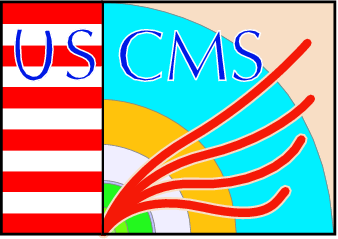
\includegraphics[height=0.6cm]{../../../Graphics/USCMS_logo.png}\hspace{.1cm}
\includegraphics[height=0.75cm]{../../../Graphics/UW_logo.png}}

\begin{document}

\begin{frame}
    \titlepage
\end{frame}

%\section{Overview}
%\begin{frame}
%    \tableofcontents
%\end{frame}

% 626 395 2112
% 421894

\section{Facilities}
\subsection{Software and Storage}
\begin{frame}
\frametitle{}
\begin{itemize}
    \item Upgraded dCache to 1.8.0-15p8
    \begin{itemize}
        \item Upgrade went well; New init script is quite handy
    \end{itemize}
    \item {\tt deploy\_srmv2.sh} failed during upgrade
    \begin{itemize}
        \item SRM mostly worked, but {\tt srm-get-metadata} failed, leading to SAM failures
        \item Created {\tt .../classes/concurrent.jar} as a zero-sized file and script completed successfully
        \item Fully upgraded SRM passes SAM
    \end{itemize}
    \item Aborted GUMS upgrade to 1.2.16
    \begin{itemize}
        \item Built hot backup service for failover
        \item Upgrade seemed successful, but still failed to {\tt generateFqanMapfile}
        \item Dan discovered that new version failed to parse user names with '\_' in them
        \item Rolled back to 1.2.10; will upgrade when OSG releases new VDT with patch
    \end{itemize}
\end{itemize}
\end{frame}

\subsection{Production and Monitoring}
\begin{frame}
\frametitle{}
\begin{itemize}
    \item SAM: OK
    \item RSV: OK
    \item JobRobot: Hmmm\ldots{}
    \begin{itemize}
        \item Good until 2008.07.21-22
        \item {\tt BrokerHelper: no compatible resources; request expired}
        \item Similar situation at other US T2s?
    \end{itemize}
    \item PhEDEx: OK
    \begin{itemize}
        \item More MC subscriptions for local users
    \end{itemize}
    \item MC Production:
    \begin{itemize}
        \item Waiting for 2\_1\_X release
        \item Testing new ProdAgent tags
    \end{itemize}
\end{itemize}
\end{frame}

\end{document}
